\chapter{The Corsican Ogre}

At the sight of this agitation Louis XVIII. pushed from him violently
the table at which he was sitting.

“What ails you, baron?” he exclaimed. “You appear quite aghast. Has
your uneasiness anything to do with what M. de Blacas has told me, and
M. de Villefort has just confirmed?” M. de Blacas moved suddenly
towards the baron, but the fright of the courtier pleaded for the
forbearance of the statesman; and besides, as matters were, it was much
more to his advantage that the prefect of police should triumph over
him than that he should humiliate the prefect.

“Sire,——” stammered the baron.

“Well, what is it?” asked Louis XVIII. The minister of police, giving
way to an impulse of despair, was about to throw himself at the feet of
Louis XVIII., who retreated a step and frowned.

“Will you speak?” he said.

“Oh, sire, what a dreadful misfortune! I am, indeed, to be pitied. I
can never forgive myself!”

“Monsieur,” said Louis XVIII., “I command you to speak.”

“Well, sire, the usurper left Elba on the 26th February, and landed on
the 1st of March.”

“And where? In Italy?” asked the king eagerly.

“In France, sire,—at a small port, near Antibes, in the Gulf of Juan.”

“The usurper landed in France, near Antibes, in the Gulf of Juan, two
hundred and fifty leagues from Paris, on the 1st of March, and you only
acquired this information today, the 3rd of March! Well, sir, what you
tell me is impossible. You must have received a false report, or you
have gone mad.”

“Alas, sire, it is but too true!” Louis made a gesture of indescribable
anger and alarm, and then drew himself up as if this sudden blow had
struck him at the same moment in heart and countenance.

“In France!” he cried, “the usurper in France! Then they did not watch
over this man. Who knows? they were, perhaps, in league with him.”

“Oh, sire,” exclaimed the Duc de Blacas, “M. Dandré is not a man to be
accused of treason! Sire, we have all been blind, and the minister of
police has shared the general blindness, that is all.”

“But——” said Villefort, and then suddenly checking himself, he was
silent; then he continued, “Your pardon, sire,” he said, bowing, “my
zeal carried me away. Will your majesty deign to excuse me?”

“Speak, sir, speak boldly,” replied Louis. “You alone forewarned us of
the evil; now try and aid us with the remedy.”

“Sire,” said Villefort, “the usurper is detested in the south; and it
seems to me that if he ventured into the south, it would be easy to
raise Languedoc and Provence against him.”

“Yes, assuredly,” replied the minister; “but he is advancing by Gap and
Sisteron.”

“Advancing—he is advancing!” said Louis XVIII. “Is he then advancing on
Paris?” The minister of police maintained a silence which was
equivalent to a complete avowal.

“And Dauphiné, sir?” inquired the king, of Villefort. “Do you think it
possible to rouse that as well as Provence?”

“Sire, I am sorry to tell your majesty a cruel fact; but the feeling in
Dauphiné is quite the reverse of that in Provence or Languedoc. The
mountaineers are Bonapartists, sire.”

“Then,” murmured Louis, “he was well informed. And how many men had he
with him?”

“I do not know, sire,” answered the minister of police.

“What, you do not know! Have you neglected to obtain information on
that point? Of course it is of no consequence,” he added, with a
withering smile.

“Sire, it was impossible to learn; the despatch simply stated the fact
of the landing and the route taken by the usurper.”

“And how did this despatch reach you?” inquired the king. The minister
bowed his head, and while a deep color overspread his cheeks, he
stammered out:

“By the telegraph, sire.” Louis XVIII. advanced a step, and folded his
arms over his chest as Napoleon would have done.

\begin{figure}[ht]
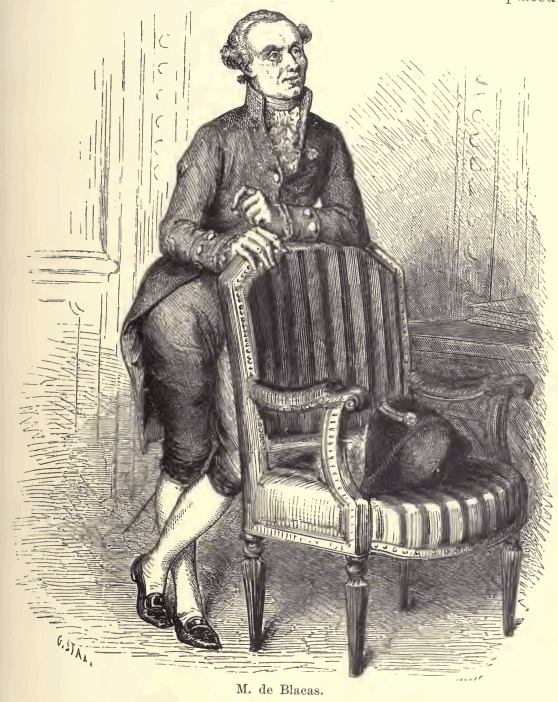
\includegraphics[width=\textwidth]{0141m.jpg}
\end{figure}

“So then,” he exclaimed, turning pale with anger, “seven conjoined and
allied armies overthrew that man. A miracle of heaven replaced me on
the throne of my fathers after five-and-twenty years of exile. I have,
during those five-and-twenty years, spared no pains to understand the
people of France and the interests which were confided to me; and now,
when I see the fruition of my wishes almost within reach, the power I
hold in my hands bursts and shatters me to atoms!”

“Sire, it is fatality!” murmured the minister, feeling that the
pressure of circumstances, however light a thing to destiny, was too
much for any human strength to endure.

“What our enemies say of us is then true. We have learnt nothing,
forgotten nothing! If I were betrayed as he was, I would console
myself; but to be in the midst of persons elevated by myself to places
of honor, who ought to watch over me more carefully than over
themselves,—for my fortune is theirs—before me they were nothing—after
me they will be nothing, and perish miserably from
incapacity—ineptitude! Oh, yes, sir, you are right—it is fatality!”

The minister quailed before this outburst of sarcasm. M. de Blacas
wiped the moisture from his brow. Villefort smiled within himself, for
he felt his increased importance.

“To fall,” continued King Louis, who at the first glance had sounded
the abyss on which the monarchy hung suspended,—“to fall, and learn of
that fall by telegraph! Oh, I would rather mount the scaffold of my
brother, Louis XVI., than thus descend the staircase at the Tuileries
driven away by ridicule. Ridicule, sir—why, you know not its power in
France, and yet you ought to know it!”

“Sire, sire,” murmured the minister, “for pity’s——”

“Approach, M. de Villefort,” resumed the king, addressing the young
man, who, motionless and breathless, was listening to a conversation on
which depended the destiny of a kingdom. “Approach, and tell monsieur
that it is possible to know beforehand all that he has not known.”

“Sire, it was really impossible to learn secrets which that man
concealed from all the world.”

“Really impossible! Yes—that is a great word, sir. Unfortunately, there
are great words, as there are great men; I have measured them. Really
impossible for a minister who has an office, agents, spies, and fifteen
hundred thousand francs for secret service money, to know what is going
on at sixty leagues from the coast of France! Well, then, see, here is
a gentleman who had none of these resources at his disposal—a
gentleman, only a simple magistrate, who learned more than you with all
your police, and who would have saved my crown, if, like you, he had
the power of directing a telegraph.” The look of the minister of police
was turned with concentrated spite on Villefort, who bent his head in
modest triumph.

“I do not mean that for you, Blacas,” continued Louis XVIII.; “for if
you have discovered nothing, at least you have had the good sense to
persevere in your suspicions. Any other than yourself would have
considered the disclosure of M. de Villefort insignificant, or else
dictated by venal ambition.” These words were an allusion to the
sentiments which the minister of police had uttered with so much
confidence an hour before.

Villefort understood the king’s intent. Any other person would,
perhaps, have been overcome by such an intoxicating draught of praise;
but he feared to make for himself a mortal enemy of the police
minister, although he saw that Dandré was irrevocably lost. In fact,
the minister, who, in the plenitude of his power, had been unable to
unearth Napoleon’s secret, might in despair at his own downfall
interrogate Dantès and so lay bare the motives of Villefort’s plot.
Realizing this, Villefort came to the rescue of the crest-fallen
minister, instead of aiding to crush him.

“Sire,” said Villefort, “the suddenness of this event must prove to
your majesty that the issue is in the hands of Providence; what your
majesty is pleased to attribute to me as profound perspicacity is
simply owing to chance, and I have profited by that chance, like a good
and devoted servant—that’s all. Do not attribute to me more than I
deserve, sire, that your majesty may never have occasion to recall the
first opinion you have been pleased to form of me.” The minister of
police thanked the young man by an eloquent look, and Villefort
understood that he had succeeded in his design; that is to say, that
without forfeiting the gratitude of the king, he had made a friend of
one on whom, in case of necessity, he might rely.

“’Tis well,” resumed the king. “And now, gentlemen,” he continued,
turning towards M. de Blacas and the minister of police, “I have no
further occasion for you, and you may retire; what now remains to do is
in the department of the minister of war.”

“Fortunately, sire,” said M. de Blacas, “we can rely on the army; your
majesty knows how every report confirms their loyalty and attachment.”

“Do not mention reports, duke, to me, for I know now what confidence to
place in them. Yet, speaking of reports, baron, what have you learned
with regard to the affair in the Rue Saint-Jacques?”

“The affair in the Rue Saint-Jacques!” exclaimed Villefort, unable to
repress an exclamation. Then, suddenly pausing, he added, “Your pardon,
sire, but my devotion to your majesty has made me forget, not the
respect I have, for that is too deeply engraved in my heart, but the
rules of etiquette.”

“Go on, go on, sir,” replied the king; “you have today earned the right
to make inquiries here.”

“Sire,” interposed the minister of police, “I came a moment ago to give
your majesty fresh information which I had obtained on this head, when
your majesty’s attention was attracted by the terrible event that has
occurred in the gulf, and now these facts will cease to interest your
majesty.”

“On the contrary, sir,—on the contrary,” said Louis XVIII., “this
affair seems to me to have a decided connection with that which
occupies our attention, and the death of General Quesnel will, perhaps,
put us on the direct track of a great internal conspiracy.” At the name
of General Quesnel, Villefort trembled.

“Everything points to the conclusion, sire,” said the minister of
police, “that death was not the result of suicide, as we first
believed, but of assassination. General Quesnel, it appears, had just
left a Bonapartist club when he disappeared. An unknown person had been
with him that morning, and made an appointment with him in the Rue
Saint-Jacques; unfortunately, the general’s valet, who was dressing his
hair at the moment when the stranger entered, heard the street
mentioned, but did not catch the number.” As the police minister
related this to the king, Villefort, who looked as if his very life
hung on the speaker’s lips, turned alternately red and pale. The king
looked towards him.

“Do you not think with me, M. de Villefort, that General Quesnel, whom
they believed attached to the usurper, but who was really entirely
devoted to me, has perished the victim of a Bonapartist ambush?”

“It is probable, sire,” replied Villefort. “But is this all that is
known?”

“They are on the track of the man who appointed the meeting with him.”

“On his track?” said Villefort.

“Yes, the servant has given his description. He is a man of from fifty
to fifty-two years of age, dark, with black eyes covered with shaggy
eyebrows, and a thick moustache. He was dressed in a blue frock-coat,
buttoned up to the chin, and wore at his button-hole the rosette of an
officer of the Legion of Honor. Yesterday a person exactly
corresponding with this description was followed, but he was lost sight
of at the corner of the Rue de la Jussienne and the Rue Coq-Héron.”
Villefort leaned on the back of an armchair, for as the minister of
police went on speaking he felt his legs bend under him; but when he
learned that the unknown had escaped the vigilance of the agent who
followed him, he breathed again.

“Continue to seek for this man, sir,” said the king to the minister of
police; “for if, as I am all but convinced, General Quesnel, who would
have been so useful to us at this moment, has been murdered, his
assassins, Bonapartists or not, shall be cruelly punished.” It required
all Villefort’s coolness not to betray the terror with which this
declaration of the king inspired him.

“How strange,” continued the king, with some asperity; “the police
think that they have disposed of the whole matter when they say, ‘A
murder has been committed,’ and especially so when they can add, ‘And
we are on the track of the guilty persons.’”

“Sire, your majesty will, I trust, be amply satisfied on this point at
least.”

“We shall see. I will no longer detain you, M. de Villefort, for you
must be fatigued after so long a journey; go and rest. Of course you
stopped at your father’s?” A feeling of faintness came over Villefort.

\begin{figure}[ht]
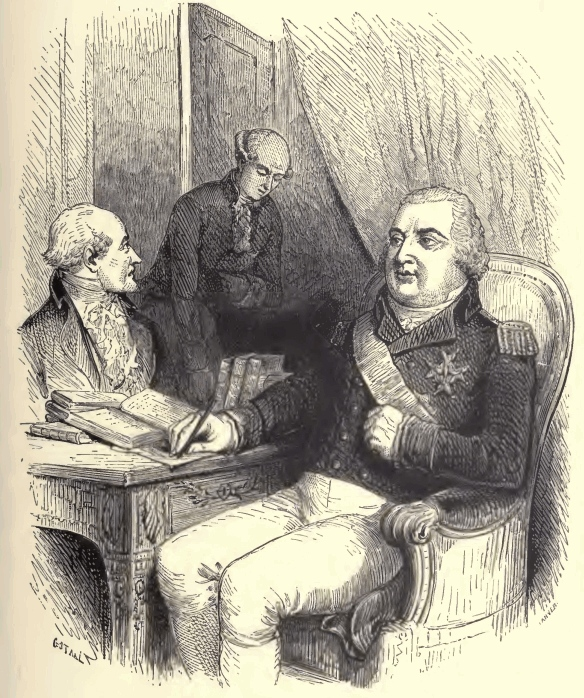
\includegraphics[width=\textwidth]{0145m.jpg}
\end{figure}

“No, sire,” he replied, “I alighted at the Hotel de Madrid, in the Rue
de Tournon.”

“But you have seen him?”

“Sire, I went straight to the Duc de Blacas.”

“But you will see him, then?”

“I think not, sire.”

“Ah, I forgot,” said Louis, smiling in a manner which proved that all
these questions were not made without a motive; “I forgot you and M.
Noirtier are not on the best terms possible, and that is another
sacrifice made to the royal cause, and for which you should be
recompensed.”

“Sire, the kindness your majesty deigns to evince towards me is a
recompense which so far surpasses my utmost ambition that I have
nothing more to ask for.”

“Never mind, sir, we will not forget you; make your mind easy. In the
meanwhile” (the king here detached the cross of the Legion of Honor
which he usually wore over his blue coat, near the cross of St. Louis,
above the order of Notre-Dame-du-Mont-Carmel and St. Lazare, and gave
it to Villefort)—“in the meanwhile take this cross.”

“Sire,” said Villefort, “your majesty mistakes; this is an officer’s
cross.”

“\textit{Ma foi!}” said Louis XVIII., “take it, such as it is, for I have not
the time to procure you another. Blacas, let it be your care to see
that the brevet is made out and sent to M. de Villefort.” Villefort’s
eyes were filled with tears of joy and pride; he took the cross and
kissed it.

“And now,” he said, “may I inquire what are the orders with which your
majesty deigns to honor me?”

“Take what rest you require, and remember that if you are not able to
serve me here in Paris, you may be of the greatest service to me at
Marseilles.”

“Sire,” replied Villefort, bowing, “in an hour I shall have quitted
Paris.”

“Go, sir,” said the king; “and should I forget you (kings’ memories are
short), do not be afraid to bring yourself to my recollection. Baron,
send for the minister of war. Blacas, remain.”

“Ah, sir,” said the minister of police to Villefort, as they left the
Tuileries, “you entered by luck’s door—your fortune is made.”

“Will it be long first?” muttered Villefort, saluting the minister,
whose career was ended, and looking about him for a hackney-coach. One
passed at the moment, which he hailed; he gave his address to the
driver, and springing in, threw himself on the seat, and gave loose to
dreams of ambition.

Ten minutes afterwards Villefort reached his hotel, ordered horses to
be ready in two hours, and asked to have his breakfast brought to him.
He was about to begin his repast when the sound of the bell rang sharp
and loud. The valet opened the door, and Villefort heard someone speak
his name.

\begin{figure}[ht]
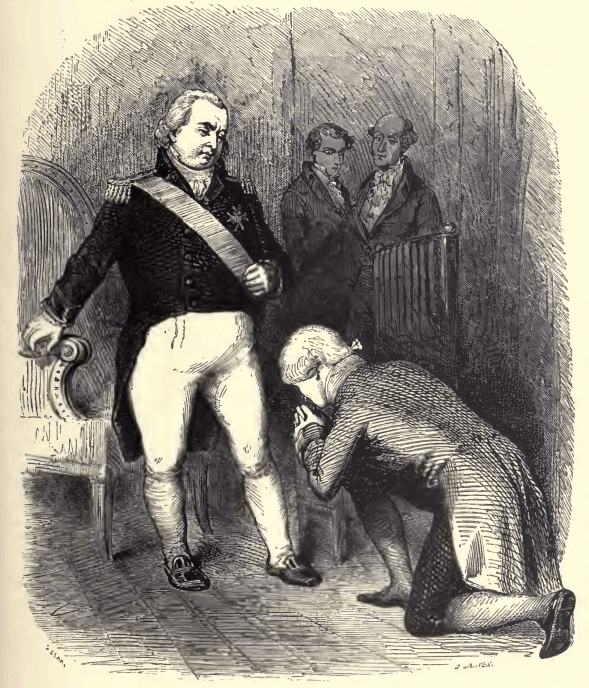
\includegraphics[width=\textwidth]{0147m.jpg}
\end{figure}

“Who could know that I was here already?” said the young man. The valet
entered.

“Well,” said Villefort, “what is it?—Who rang?—Who asked for me?”

“A stranger who will not send in his name.”

“A stranger who will not send in his name! What can he want with me?”

“He wishes to speak to you.”

“To me?”

“Yes.”

“Did he mention my name?”

“Yes.”

“What sort of person is he?”

“Why, sir, a man of about fifty.”

“Short or tall?”

“About your own height, sir.”

“Dark or fair?”

“Dark,—very dark; with black eyes, black hair, black eyebrows.”

“And how dressed?” asked Villefort quickly.

“In a blue frock-coat, buttoned up close, decorated with the Legion of
Honor.”

“It is he!” said Villefort, turning pale.

\begin{figure}[h]
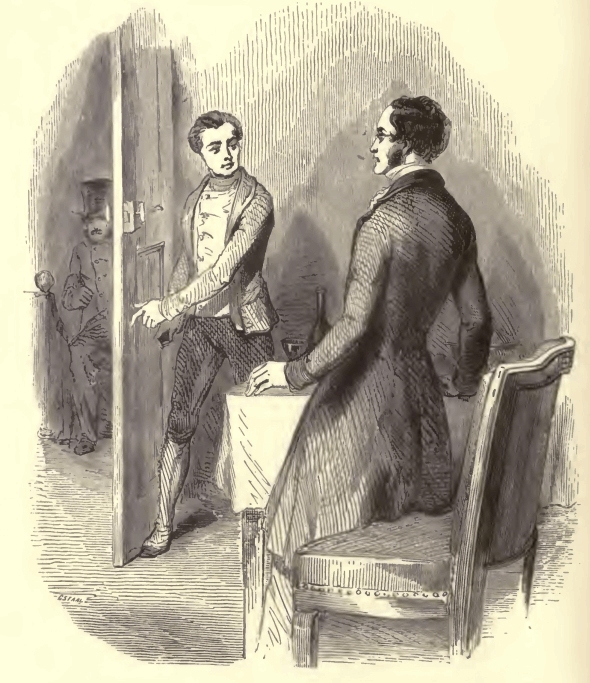
\includegraphics[width=\textwidth]{0148m.jpg}
\end{figure}

“Eh, \textit{pardieu!}” said the individual whose description we have twice
given, entering the door, “what a great deal of ceremony! Is it the
custom in Marseilles for sons to keep their fathers waiting in their
anterooms?”

“Father!” cried Villefort, “then I was not deceived; I felt sure it
must be you.”

“Well, then, if you felt so sure,” replied the new-comer, putting his
cane in a corner and his hat on a chair, “allow me to say, my dear
Gérard, that it was not very filial of you to keep me waiting at the
door.”

“Leave us, Germain,” said Villefort. The servant quitted the apartment
with evident signs of astonishment.
